% THIS IS SIGPROC-SP.TEX - VERSION 3.1
% WORKS WITH V3.2SP OF ACM_PROC_ARTICLE-SP.CLS
% APRIL 2009
%
% It is an example file showing how to use the 'acm_proc_article-sp.cls' V3.2SP
% LaTeX2e document class file for Conference Proceedings submissions.
% ----------------------------------------------------------------------------------------------------------------
% This .tex file (and associated .cls V3.2SP) *DOES NOT* produce:
%       1) The Permission Statement
%       2) The Conference (location) Info information
%       3) The Copyright Line with ACM data
%       4) Page numbering
% ---------------------------------------------------------------------------------------------------------------
% It is an example which *does* use the .bib file (from which the .bbl file
% is produced).
% REMEMBER HOWEVER: After having produced the .bbl file,
% and prior to final submission,
% you need to 'insert'  your .bbl file into your source .tex file so as to provide
% ONE 'self-contained' source file.
%
% Questions regarding SIGS should be sent to
% Adrienne Griscti ---> griscti@acm.org
%
% Questions/suggestions regarding the guidelines, .tex and .cls files, etc. to
% Gerald Murray ---> murray@hq.acm.org
%
% For tracking purposes - this is V3.1SP - APRIL 2009

\documentclass{acm_proc_article-sp}

\begin{document}

\title{Spring XD: A Modular Distributed Stream and Batch Processing System}

% You need the command \numberofauthors to handle the 'placement
% and alignment' of the authors beneath the title.
%
% For aesthetic reasons, we recommend 'three authors at a time'
% i.e. three 'name/affiliation blocks' be placed beneath the title.
%
% NOTE: You are NOT restricted in how many 'rows' of
% "name/affiliations" may appear. We just ask that you restrict
% the number of 'columns' to three.
%
% Because of the available 'opening page real-estate'
% we ask you to refrain from putting more than six authors
% (two rows with three columns) beneath the article title.
% More than six makes the first-page appear very cluttered indeed.
%
% Use the \alignauthor commands to handle the names
% and affiliations for an 'aesthetic maximum' of six authors.
% Add names, affiliations, addresses for
% the seventh etc. author(s) as the argument for the
% \additionalauthors command.
% These 'additional authors' will be output/set for you
% without further effort on your part as the last section in
% the body of your article BEFORE References or any Appendices.

\numberofauthors{5} %  in this sample file, there are a *total*
% of EIGHT authors. SIX appear on the 'first-page' (for formatting
% reasons) and the remaining two appear in the \additionalauthors section.
%
\author{
% You can go ahead and credit any number of authors here,
% e.g. one 'row of three' or two rows (consisting of one row of three
% and a second row of one, two or three).
%
% The command \alignauthor (no curly braces needed) should
% precede each author name, affiliation/snail-mail address and
% e-mail address. Additionally, tag each line of
% affiliation/address with \affaddr, and tag the
% e-mail address with \email.
%
% 1st. author
\alignauthor Sabby Anandan
% 2nd. author
\alignauthor Marius Bogoevici
% 3rd. author
\alignauthor Glenn Renfro
\and  % use '\and' if you need 'another row' of author names
% 4th. author
\alignauthor Ilayaperumal Gopinathan
% 5th. author
\alignauthor Patrick Peralta
}
% There's nothing stopping you putting the seventh, eighth, etc.
% author on the opening page (as the 'third row') but we ask,
% for aesthetic reasons that you place these 'additional authors'
% in the \additional authors block, viz.

% Just remember to make sure that the TOTAL number of authors
% is the number that will appear on the first page PLUS the
% number that will appear in the \additionalauthors section.

\maketitle
\begin{abstract}
Spring XD is a unified, distributed, and extensible system for data ingestion, real time analytics, batch processing, and data export. The project's goal is to simplify the development of big data applications.
NOTE: THIS IS COPY/PASTED FROM WEB SITE; SHOULD BE REVIEWED.
\end{abstract}

\section{Introduction}

The era of Big Data has introduced many new technologies for data storage
and processing. The success and high demand for horizontally scalable
solutions such as HDFS, Spark, and Kafka demonstrates this need. At the
same time, enterprises have invested heavily in older and proven
technologies such as SQL databases and messaging systems. For enterprises
to adopt the emerging technologies, there must be a way to easily
connect with existing systems.

Since its inception in 2004, the main objective of the Spring Framework
has been to simplify application development. At the time, Java developers
were struggling with EJBs, boilerplate JDBC, and JMS. Today's developers
are dealing with an explosion of data and the leading-edge tools to
manage and process this data.

Expanding upon the success of existing technologies in the Spring portfolio
such as Spring Integration and Spring Batch, Spring XD provides a runtime
environment that integrates with a plethora of technologies, both established
and up-and-coming.

Although enterprise system integration is one of the strengths of Spring XD,
it is a compelling technology for brand new applications that have streaming
or batch data processing requirements. Spring XD features a built in
interactive shell for creating streams or jobs without writing any Java code.
This allows for quick development cycles and easy experimentation.

Creating a stream in Spring XD is a simple concept for those familiar with
UNIX streams and pipes. Consider the following shell command:

\verb;tail -f /tmp/log.txt | grep ERROR;

The tail command will continuously display the file contents. The |
will pipe the output of tail to grep, which will filter out all
lines that do not contain the string ERROR.

The equivalent using Spring XD looks like this:

\verb;stream create -name error-filter -definition;\\*
\verb;  "tail -name=/tmp/log.txt | filter;\\*
\verb;  --expression=payload.contains('ERROR') | log";

While this specific example will only tail a local file, a distributed 
ingestion stream that aggregates, filters, and stores log file analytics
can just as easily be created with Spring XD.


\section{Architecture}
This section describes the internal architecture of Spring XD. See figure~\ref{fig:architecture}.

\subsection{Application Context}
The foundation of Spring XD is the Spring application context. The application context is a dependency injection framework that is used to instantiate objects along with their dependencies \cite{spring-framework-reference}. 

\subsection{Modules}


\begin{figure}[ht]
\centering
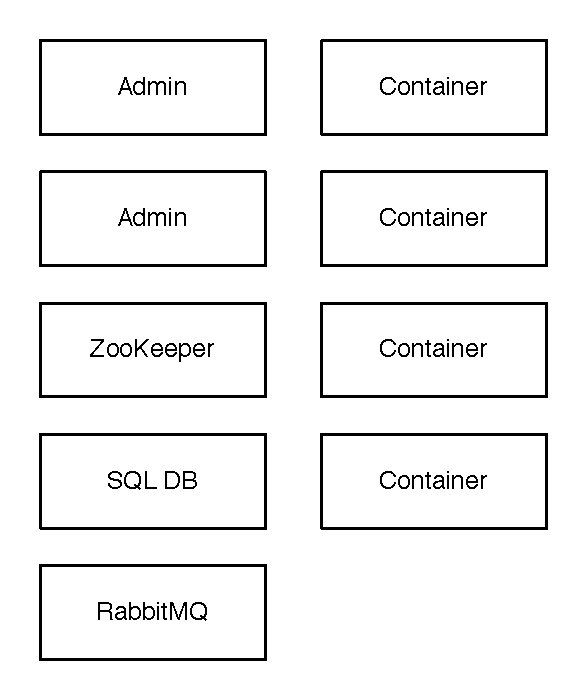
\epsfig{file=XD-sample.eps, height=2in, width=2in}
\caption{Spring XD Architecture.}
\label{fig:architecture}
\end{figure}

Here is where we get into the fine grained details.

\section{Deployment}
This section describes deployment architectures with Spring XD.
\subsection{Lambda architecture}

The Lambda Architecture, introduced by Nathan Marz \cite{lambda-architecture-paper} is a generic, scalable and fault tolerant data processing archictecture. It attempts to provide a comprehensive solution to the problem of processing an extremely large set of data.


The Lambda Architecture has the following components:

\begin{itemize*}
\item A \emph{master dataset} comprising of all data known to the system, ideally in its rawest form;
\item A \emph{serving} or \emph{view layer} that provides the latest, most up-to-date view of the processed data, available for low-latency, ad-hoc querying;
\item A \emph{batch layer} that performs computationally intense calculations that and prepares the \emph{batch views} displayed by the \emph{serving layer};
\item A \emph{speed layer} that performs calculations on recent data only, its output combined with the \emph{batch views} by the \emph{serving layer}.
\end{itemize*}

The guiding principle of the Lambda architecture is an attempt to combine the high throughput of batch operations with the low latency of real-time computations. Each on its own, has its strenghts and weakness. While the highest throughput for computing large datasets is attained by relying on batch computations, the latter have the disadvantage of higher latency. Meanwhile, real-time computations may operate with low latency and produce results based on latest data quickly, but can't really handle the large amounts of data that batch processing can deal with. So, instead of relying on a single paradigm, the lambda architecture employs both, allowing them to complement each other.

A detailed view of the Lambda Architecture can be viewed in figure [TBD]

\subsubsection {Master dataset in Spring XD}

While Spring XD does not provide a storage mechanism of its own, it integrates with a variety of data sources, allowing both reading (through its source[reference tbd, provide example] components), as well as writing, through its sink[reference tbd, provide examples] components. As such, it provides all the necessary means for ingesting data into a master dataset, also allowing for consolidating data from a variety of sources. 

TBD: provide an example of a simple stream

TBD: provide example of multiple streams with a namd queue sink and a stream with a named queue source. By sharing the sink, we create the master dataset out of multiple sources.

\subsubsection {Speed layer in Spring XD}

The Speed layer in Spring XD is handled by the streams. Transformers. Illustrate transformation of data, aggregation via counters.  

\subsubsection {Batch layer in Spring XD}

Jobs.

\subsubsection {Combining the two}

Stream-driven batch jobs. Taps. 

\subsubsection {View layer in Spring XD}

Externalized via sinks, output of batch jobs. Microservice architecture Example of a web application reading data off a set of tables written on by Spring XD. 

\subsubsection {Critique of the Lambda Architecture and Spring XD}

An often raised objection to the LA is the duplication of work (Quote Jay Kreps) that occurs during processing. More specifically, the necessity of writing the same processing code twice: once for the speed and once for the batch layer. However, due to the nature of Spring XD, the same business code can be shared between the two layers. This objection does not apply!


\subsection {Reactive architectures}

\subsection {Cloud deployment - does this even belong here??}


\section{Integrations}
Spring XD integration modules are Message Endpoints \cite{enterprise-inetgration-pattern} that responsible for sending to and receiving data from external agents.  There are 3 types of message endpoints: Source, Sinks and Batch Jobs.  The source's responsibility is to receive the inbound data and convert it to a message that will be used by modules in the stream(reference streams) or by a job that is launched based on the receipt of the data.  The sink's responsibility is to convert the message to the format that can be consumed by the external agent and transmit the data to the agent.   Batch Jobs may be used to execute specialized logic on a large set of data from one external agent and transmit the resulting data to another external agent.  Spring XD offers a suite of 23 sources (file, jdbc, Mongo, HDFS, \ldots), 24 sinks (file, jdbc, Mongo, HDFS, \ldots) and 9 jobs (filepollhdfs, sparkapp, sqoop, \ldots)  that are ready to use at XD startup.  
If an existing module does meet the needs of for the given use case a user may create a custom integration module.\par
A source's responsibility is to receive the inbound data and convert it to a message for use by modules in a stream or by a batch job.  There are 2 types of source: Poller and Socket.  A poller source will interrogate an external agent for data at a interval specified by the user.  A socket source will have a port open ready to receive data that is pushed from an external agent.  \par
 There are 2 types of sinks: Counter/gauge and Delegate.  A counter/gauge is a specialized sink increments a field on a datastore every time a message is received refer to the (Analytics Section) for more information.  As a delegate sink's responsibility is to translate the XD message to the format that can be used by the external agent and dispatch that data to the agent.  
	A batch job's responsibility is to read and or write of data from an external agent, execute a migration of data that needs transactional safeguards or to execute an external process (SparkApp). \par
Use Cases 
With the advent of microservices \cite{microservices-pattern} applications are becoming evermore integrated.  In cases where an agent needs access to microservices but does not have the capability to transmit the request via the API presented, or an agent needs to take the results of a microservice and transmit it to  an external agent in the agent's accepted format, XD can bridge that chasm. 
An example of this would be if we needed a service that would receive sensor data via mqtt and write that the data to hdfs. The following stream would be used to do this: "mqtt|hdfs".
Another example of this would be a scenario if a database is being updated by an service but while the database is updated we need to update a collection in a mongo collection with this data.  This can be done by creating a stream that would monitor a table(s) retrieve changes and write the results to the mongo collection.  This would be respresented by the following stream: "jdbc --fixedDelay=1 --split=1 --query='select * from testfoo where tag = 0' --update='update testfoo set tag=1 where fooid in (:fooid)'|log" \par
Example Source
jdbc - is a poller source that will execute a query against a database and generate a message for each row that is retrieved.  \cite{jdbc-module}
mqtt - is a socket source that awaits for mqtt messages to be received once the message is received the payload of the message is sent as an XD message to the next module in the stream.  \cite{mqtt-module}
Example Sink
Mongo - The Mongo sink writes messages into a Mongo collection \cite{mongo-module}
hdfs - writes messages to the specified location on a hadoop instance. \cite{hadoop-hdfs-module}
Example Job
filejdbc -A module which loads CSV files into a JDBC table

Integration Modules are deployed in the modules subdirectory and are segregated in subdirectories by type: modules/source, modules/sink and modules/job.  
These modules are dynamically loaded when a stream or job is created that requires that specific module.  Once loaded, they are stored in Java's classloader and will not be reloaded (until the XD container is restarted).  Besides the pre-existing integration modules that come with the XD installation a user may create their own integration modules. \par

Spring XD uses Spring Integration \cite{spring-integration-reference} as its foundation for implementing source, sink and batch modules.  As such integration modules are comprised minimally of one channel and a integration bean.  In the case of a source module there is an "output" channel to dispatch messages transmitted by the integration bean to the stream figure~\ref{fig:sourcembc}. 
\begin{figure}[ht]
\centering
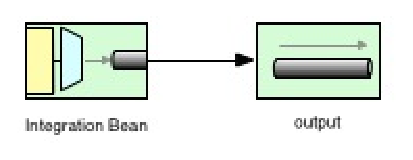
\epsfig{file=integration-module-output-channel.eps, height=.8in, width=2in}
\caption{Source Module Basic Components}
\label{fig:sourcembc}
\end{figure}

 For a sink there is an "input" stream for which all messages from the stream will be dispatched and then read by the integration bean figure~\ref{fig:sinkmbc}. 

\begin{figure}
\centering
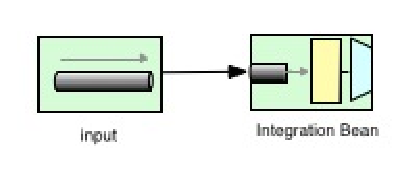
\epsfig{file=integration-module-input-channel.eps, height=.8in, width=2in}
\caption{Sink Module Basic Components}
\label{fig:sinkmbc}
\end{figure}

Current end. \par

\section{Use Cases}
Few Fortune 100 and several Fortune 1000 companies are using Spring XD but all are under NDA. Following are some of the common use-cases that we have been supporting in the field.

\begin{itemize*}
\item \textbf{Fault Detection}: Spring XD connects machine data with enterprise infrastructure, middleware, and backend services. Continuous streams can be orchestrated in Spring XD to connect with various devices (i.e., machines). Consume and transform data of varied formats, analyze, predict failures, generate reports, and dispatch maintenance personnel - all in real-time.
\item \textbf{Enterprise Modernization}: Enterprises invest heavily on IT infrastructure, as the data resides at several layers in the enterprise architecture. Tight coupling with various products further adds more overhead with data management. Spring XD, as one-stop runtime, provides data integration adapters to consume data of varied formats (i.e., structures, unstructured, binary, ..) that reside in different toolchains (i.e., database, middlewares, in-memory grids, ..). Given the unified approach, enterprises' are equipped with developer-friendly fixtures to create pipelines using Spring XD. Pipelines connecting varied data producing and consuming agents eliminates the necessity of toolchains, maintenance overhead, or production support - Spring XD simplifies data collection and aggregation.
\item \textbf{Data Ingest}: Spring XD is a standard tool for ingesting data into Hadoop. Whether it is real-time (i.e., online) or batch (i.e., offline), you've fixtures to operationalize pipeline that fits your business needs.
\item \textbf{24/7 Production Pipelines}: The business demands highly available data streams with guaranteed data processing, to react in real-time accurately. Spring XD's runtime is highly reliable that can recover from failures seamlessly. Production running pipelines are long running tasks - there's no end. For ad-hoc operations such as querying, machine learning, or data crunching, `taps' in Spring XD are commonly adopted to fork the data from primary pipeline. This results in no disruption with the primary pipeline, at the same time ad-hoc demands can be fulfilled. 
\item \textbf{Closed-loop Analytics}: Spring XD orchestrates the entire analytics loop - gathering data from any source, triggering actions, handling feedback loops from machine learning models, and computing real-time predictions.
\item \textbf{Hadoop and Beyond}: Enterprises with existing investment in Hadoop technologies find Spring XD as one-stop orchestration platform. Whether it is MapReduce, Hive, Pig, or HBase scripts - developer experience is the same.
\end{itemize*}


\section{Related Work}
This section compares and contrasts Spring XD to similar projects.

\subsection{Spring XD and Spark}
Spark\cite{spark} is a general-purpose framework for large scale data processing.
In comparison with Hadoop's disk based MapReduce programming model, Spark's 
in-memory primitives provide immediate performance improvements.

The following features differentiate Spring XD and Spark Streaming.

\begin{itemize*}
\item Readily available integration adapters for data movements from various 
data sources in to Hadoop and others.
\item Ability to microbatch based on event count via Reactor and RxJava APIs.
\item Ability to create data pipelines to process one event at a time.
\item Flexibility to specify hosts to dictate the location of data computations.
\end{itemize*}

The following features differentiate Spring XD and Spark Batch processing.

\begin{itemize*}
\item Provides REST-API and lifecycle management for Spark jobs.
\item Extensible to integrate with other Batch systems.
\end{itemize*}

Recognizing the strengths of distributed data computations with Spark, Spring XD 
supports integration with Spark applications such as Spark Streaming, MLLib, and 
SparkSQL. Users familiar with Spark may implement the computation logic using 
Spark APIs in Java or Scala, and leave the orchestration to Spring XD. 
Spring XD also adds value by restarting the Spark Streaming driver to recover 
from fault scenarios.

\subsection{Spring XD and Storm}
Apache Storm\cite{storm} is a distributed computation system for real time stream 
processing.

The following features differentiate Spring XD and Storm.

\begin{itemize*}
\item Spring XD provides interactive Shell as opposed to Storm's API model to
create data pipelines.
\item Use of `taps' in Spring XD to build stream pipelines in isolation
without having to disrupt existing pipelines.
\item Loosely coupled `modules' in Spring XD are responsible for ingestion, analytics, 
data processing, machine learning or data export. Modules can be individually managed 
and dynamically scaled.
\item The notion of `composite modules' (unit\-of\-work) and colocation 
capabilities to fine-tune performance characteristics. 
\item Building upon the functional stream processing model, users have the option 
to choose from Reactor\cite{reactor}, Spark Streaming or RxJava APIs, to build 
complex data centric applications.
\end{itemize*}

Storm and Spring XD supports many common data sources and middleware's. 
For example, you can read and write data payloads from Apache Kafka topics both 
in Storm and Spring XD. Bolts/Spouts in Storm is analogous to Source/Processor/Sink 
in Spring XD. As stream processing frameworks, Storm and Spring XD can be used for 
similar use-cases.

\subsection{Spring XD and Flume}
Apache Flume\cite{flume} is a distributed system for collecting, aggregating and 
moving large data sets. 

The following features differentiate Spring XD and Flume.

\begin{itemize*}
\item High-level DSL to build streams and jobs.
\item Ability to monitor data workflows either via DSL, Admin UI, or custom 
dashboards.
\item Administer data pipelines through Admin UI.
\item Granular controls to manifest batch job and step execution to create 
complex data driven workflows.
\item Flexibility through `Deployment Manifest' to declaratively configure data 
partitioning strategy to route data to a specific consumer instance in the cluster.
\end{itemize*}

Flume offers HBase, Solr, and ElasticSearch sinks along with encryption support 
for Avro sources, which we are planning to address in our future releases.

\subsection{Spring XD and Oozie}
Oozie\cite{oozie} is a workflow scheduler engine to manage Hadoop \cite{hadoop} 
workloads such as MapReduce or Pig jobs. 

The following features differentiate Spring XD and Oozie.

\begin{itemize*}
\item Building upon Spring Batch, a JSR standardization (JSR-352) of batch 
workload data processing, Spring XD inherits workflow scheduling and execution 
functionaliites.
\item Provides out of the box batch jobs such as file-to-jdbc, file-to-hdfs, 
ftp-to-hdfs, hdfs-to-jdbc, hdfs-to-mongo, jdbc-to-hdfs, spark-job, and sqoop-job.
\item Ability to scale jobs without having to bring down the runtime.
\item Provides bidirectionality between real-time streaming and batch 
workflows to accommodate complex data processing use cases.
\item Ability to create and launch workflow-jobs from Admin UI. 
\item Ability to view historical snapshots of job executions from Admin UI.
\end{itemize*}

Oozie offers HCatalog integration, which we are planning to address in our 
future releases.

\subsection{Spring XD and Sqoop}
Apache Sqoop\cite{sqoop} assists with data transmission between Hadoop and relational 
databases.

The following features differentiate Spring XD and Sqoop.

\begin{itemize*}
\item Ability to orchestrate Pig, Hive, HBase, MapReduce or other batch systems.
\item Flexibility to extend batch workflow infrastructure to write custom tasklets.
\item High level configuration DSL to create, deploy and destroy batch workflows.
\item Flexibility to operationalize custom data pipelines through REST-APIs.
\item Unified functional programming support to build reactive-style data pipelines.
\end{itemize*}

Sqoop offers data validation, data merge, incremental data imports, and HCatalog 
integration among others. Recognizing the importance of these enterprise features, 
Spring XD provides an out of the box Sqoop job to take advantage and orchestrate 
data movements.

\section{Conclusion}

Mission critical data applications cannot live in a vacuum. The abundance of data
and specialized applications to process and store it require a holistic approach.
Spring XD is a formidable solution for managing the data flow and processing
between these applications. Spring XD integrates with systems ranging from decades
old RDBMS to cutting edge Big Data. The suite of Spring Framework projects that
Spring XD builds upon allows for flexible extensibility. The distributed runtime
built on ZooKeeper provides reliability and scale out capabilities for streams
and jobs. 


%\end{document}  % This is where a 'short' article might terminate

%ACKNOWLEDGMENTS are optional
\section{Acknowledgments}
This section is optional; it is a location for you
to acknowledge grants, funding, editing assistance and
what have you.  In the present case, for example, the
authors would like to thank Gerald Murray of ACM for
his help in codifying this \textit{Author's Guide}
and the \textbf{.cls} and \textbf{.tex} files that it describes.

%
% The following two commands are all you need in the
% initial runs of your .tex file to
% produce the bibliography for the citations in your paper.
\bibliographystyle{abbrv}
\bibliography{sigproc}  % sigproc.bib is the name of the Bibliography in this case
% You must have a proper ".bib" file
%  and remember to run:
% latex bibtex latex latex
% to resolve all references
%
% ACM needs 'a single self-contained file'!
%
%APPENDICES are optional
%\balancecolumns
\appendix
%Appendix A
\section{Headings in Appendices}
The rules about hierarchical headings discussed above for
the body of the article are different in the appendices.
In the \textbf{appendix} environment, the command
\textbf{section} is used to
indicate the start of each Appendix, with alphabetic order
designation (i.e. the first is A, the second B, etc.) and
a title (if you include one).  So, if you need
hierarchical structure
\textit{within} an Appendix, start with \textbf{subsection} as the
highest level. Here is an outline of the body of this
document in Appendix-appropriate form:
\subsection{Introduction}
\subsection{The Body of the Paper}
\subsubsection{Type Changes and  Special Characters}
\subsubsection{Math Equations}
\paragraph{Inline (In-text) Equations}
\paragraph{Display Equations}
\subsubsection{Citations}
\subsubsection{Tables}
\subsubsection{Figures}
\subsubsection{Theorem-like Constructs}
\subsubsection*{A Caveat for the \TeX\ Expert}
\subsection{Conclusions}
\subsection{Acknowledgments}
\subsection{Additional Authors}
This section is inserted by \LaTeX; you do not insert it.
You just add the names and information in the
\texttt{{\char'134}additionalauthors} command at the start
of the document.
\subsection{References}
Generated by bibtex from your ~.bib file.  Run latex,
then bibtex, then latex twice (to resolve references)
to create the ~.bbl file.  Insert that ~.bbl file into
the .tex source file and comment out
the command \texttt{{\char'134}thebibliography}.
% This next section command marks the start of
% Appendix B, and does not continue the present hierarchy
\section{More Help for the Hardy}
The acm\_proc\_article-sp document class file itself is chock-full of succinct
and helpful comments.  If you consider yourself a moderately
experienced to expert user of \LaTeX, you may find reading
it useful but please remember not to change it.
\balancecolumns
% That's all folks!
\end{document}
